\chapter{Background}
    This chapter aims to provide firstly a complete background of the concepts key to understanding the $\Delta$QSD paradigm.

    Secondly, we provide a comprehensive background into the observability solutions that have been explored for the oscilloscope, delving deeper into OpenTelemetry and its macros.
    
    We finish by explaining what we believe are the current limitations of OpenTelemetry and explaining where the paradigm and the oscilloscope comes in.
    
    \section{An overview of $\Delta$QSD}
    $\Delta$QSD is a metrics-based, quality-centric paradigm that uses formalised outcome diagrams to explore the performance consequences of design decisions. \cite{myo}
    
    Key concepts of $\Delta$QSD are \textbf{quality attenuation ($\Delta$Q)} and \textbf{outcome diagrams} \cite{dq-tut}.

    Outcome diagrams capture dependency and causality properties of the system. The $\Delta$QSD paradigm derives bounds on performance expressed as probability distribution, encompassing all possible executions of the system. \cite{myo}
 
    The following sections are a summary of multiple articles and presentations formalising the paradigm.
     
 \subsection{Outcome}
           An outcome $o$ is a specific system behaviour that can be observed to start at some point in time and \textit{\textbf{may}} be observed to complete at some later time. \cite{dq-br}
        Formally, what the system obtains by performing one of its tasks. One task corresponds to one outcome and viceversa. When an outcome is performed, it means that the task of an outcome is performed.
     
        The particularity of outcomes is that they can represent multiple levels of granularity. Suppose an outcome is beyond the current system's control (e.g. a database/cloud request), is non-atomic (can be broken down in multiple sub-outcomes). These outcomes can be represented as black-boxes (you can observe their start and end, but do not know what is being executed). As the system gets refined, these outcomes can then be refined to model a single outcome or multiple outcomes, if needed. \\ 
        Even though these outcomes are defined as "black boxes", they still have timeliness constraints like any other outcome. \cite{myo}

     \paragraph{Observables}
    Each outcome has two starting sets of events: the starting sets and the ending sets. Such sets are called the \textit{observables}. Once an event from the starting set occurs, there is no guarantee that a corresponding event in the terminating set will occur within the duration limit (required time to complete). An observable is \textit{done} when it occurs during the time limit. \cite{art}

    \paragraph{Outcome instance}
    An outcome instance is the result of an execution of an outcome given a starting event $e_{in}$ and an end event $e_{out}$. \cite{art}

    \paragraph{Graphical Representation}
    Outcomes are represented as circles, with the starting and terminating set of events being represented by boxes.
    \begin{figure}[H]
        \begin{center}
            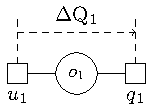
\includegraphics[scale=1.2]{tikz/outdq.pdf}
        \end{center}
        \caption{The outcome (circle) and the starting set (left) and terminating set (right) of events. \cite{myo}}
    \end{figure}

\subsection{Quality attenuation ($\Delta$Q)}
        Assume a component $C$ which receives a message $m_{in}$ and outputs a message $m_{out}$ after a delay $d$. Over multiple executions, we will have observed multiple delays which can be represented as a cumulative definition where $p$ percent of delays have delay $\le d$. \cite{art} 

        \textbf{$\Delta$Q} is a cumulative distribution function that defines both \textit{latency} and \textit{failure probability} between a start and end event. \cite{dq-tut}

        In an ideal system, an outcome would deliver a desired behaviour without error, failure, delay, but this is not the case. The quality of an outcome response "attenuated to the relative ideal" (the cumulative distribution function) is called "quality attenuation" ($\Delta$Q) and can depend on many factors (geographical, physical \dots). Its distribution may be modelled by a random variable.

    As $\Delta$Q captures deviation from ideal behavior and incorporates delay, which is a continuous random variable, and failures/timeouts, which are discrete variables, it can be described mathematically as an \textit{Improper Random Variable}, where the probability of a finite or bounded delay $<$ 1. 

    \textbf{$\Delta$Q(x)} is the probability that an outcome $O$ occurs in time $t \le x$. The \textbf{\textit{intangible mass}} $1 - \lim_{x\to\infty}\Delta Q(x)$ of a $\Delta$Q will encode the probability of failure/timeout/exception occuring. \cite{myo}
    
    \begin{figure}[H]
        \begin{center}
            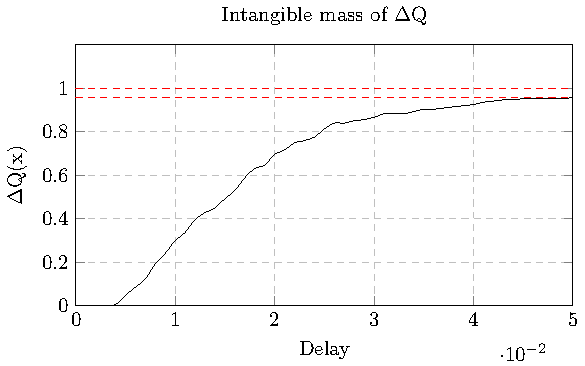
\includegraphics{tikz/intangible.pdf}
        \end{center}
        \caption{Intangible mass (red) of a $\Delta$Q with failure rate of about 5\% }
    \end{figure}
   
  \subsection{Failure semantics}
       In the CDF representation of a $\Delta$Q, there is an \textit{f} percent probability that the delay is infinite, this is what failure models. 
        Concretely, it means that an input message $m_{in}$ \textbf{has no output message} $m_{out}$. \cite{art}

        Combining delay and failure in a single quantity is what makes $\Delta$QSD a great choice to explore feasibility in system design. \cite{dq-tut}
   
    \subsection{Partial ordering}
        A CDF of a $\Delta$Q is \textit{less than} the other if its CDF is everywhere to the left and above the other. Mathematically, it is a partial order. 
        
        If two $\Delta$Qs intersect, they are not ordered. \cite{dq-tut}

    \subsection{Timeliness}
        Timeliness is defined as a relation between an observed $\Delta Q_{obs}$ and a required $\Delta Q_{req}$. Timeliness is delivering results within required time bounds (sufficiently often). 

        A system \textit{satisfies timeliness} if $\Delta$Q$_{obs}$ $\le$ $\Delta$Q$_{req}$. \cite{art}
     
    \subsection{QTA, required $\Delta$Q}
         The \textit{Quantitative Timeliness Agreement} (QTA) maps objective measurements to the subjective perception of application performance. It specifies what the base system does and its limits. \cite{dq-br}
    
    \paragraph{Slack} There is performance \textit{slack} when a $\Delta$Q is strictly less than the requirement,

        \paragraph{Hazard} There is performance \textit{hazard} when a $\Delta$Q is strictly greater than the requirement. \cite{myo}
    
    \paragraph{QTA example}: Imagine a system where 25\% of the executions should take $<$ 15 ms, 50\% $<$ 25 ms and 75\% $<$ 35 ms, all queries have a maximum delay of 50ms and 5\% of executions can timeout, the QTA can be represented as a step function.
    
        \begin{figure}[H]
            \begin{center}
                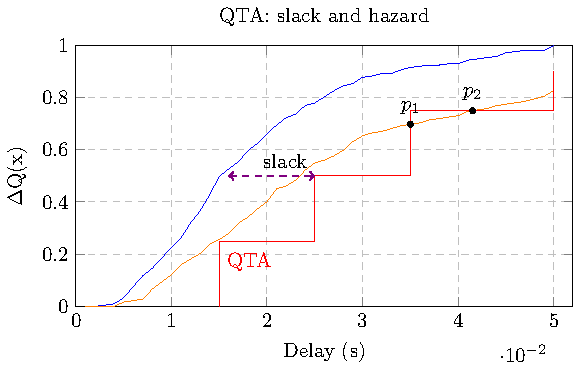
\includegraphics[scale=1]{tikz/cdf_qta_slack.pdf}
            \end{center}
            \caption{The system in blue is showing slack and satisfies the requirement. The system in orange is showing signs that it cannot handle the stress, it is not respecting the system requirements imposed by the QTA.}%
        \end{figure}

    \subsection{Outcome diagram}
        An outcome diagram is central to capture the causal relationships between the outcomes. It shows the causal connections between all the outcomes we are interested in, and it allows computing the $\Delta$Q for the whole system \cite{dq-tut}. It maps a system's behaviour as seen from outside to concrete outcomes \cite{art}.
        There are four different operators that represent the relationships between outcomes. \cite{dq-tut}

    \subsubsection{Sequential composition}
        If we assume two outcomes $O_A$, $O_B$ where the end event of $O_A$ is the start event of $O_B$, the two outcomes can be sequentially composed. The total delay $\Delta$Q$_{AB}$ is given by the convolution of the PDFs of $O_A$ and $O_B$ ($O_A \circledast O_B$).
        
        \begin{figure}[H]
            \begin{center}
                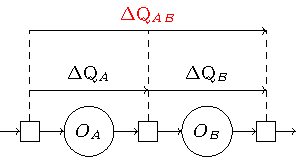
\includegraphics[scale=1]{tikz/seq_comp.pdf}
            \end{center}
            \caption{Sequential composition of $O_A$ and $O_B$.}
        \end{figure}
        Where convolution ($\circledast$) between two PDF is:
        \begin{equation}
            PDF_{AB}(t) =\int\limits_0^t PDF_A(\delta) \cdot PDF_B(t-\delta)d\delta 
            \label{eq:conv_1}
        \end{equation}

        Thus, $\Delta$Q$_{AB}$:
        \begin{equation}
            \Delta Q_{AB} = PDF_{A} \circledast PDF_{B}
            \label{eq:convolution_pdf}
        \end{equation}

        Convolution is the only operation which is based on the PDFs, the following operations are based on the CDF of the $\Delta$Qs (hence the use of the $\Delta$Q notation).
        
    \subsubsection{First to finish (FTF)}
            If we assume two independent outcomes $O_A$, $O_B$ with the same start event, first-to-finish occurs when at least one end event occurs, it can be calculated as:
        \begin{equation}
            \begin{split}
                \Delta Q_{FTF(A, B)} &= Pr[d_A > t \wedge d_B > t] \\
                & = Pr[d_A > t] \cdot Pr[d_B > t] = (1 - \Delta Q_A) \cdot (1 - \Delta Q_B) \\
                \Delta Q_{FTF(A, B)} &= \Delta Q_A + \Delta Q_B - \Delta Q_A \cdot \Delta Q_B  
            \end{split}    
            \label{eq:ftf} 
        \end{equation}

       \begin{figure}[H]
            \centering
            \begin{subfigure}{.5\textwidth}
                \centering
                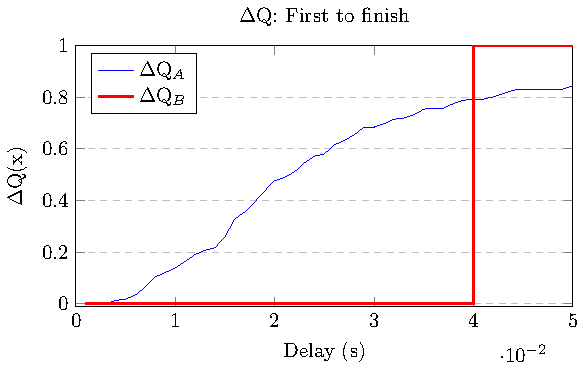
\includegraphics[scale = 0.7]{tikz/ftf_1.pdf}
                \label{fig:ftf1}
            \end{subfigure}%
            \begin{subfigure}{.5\textwidth}
                \centering
                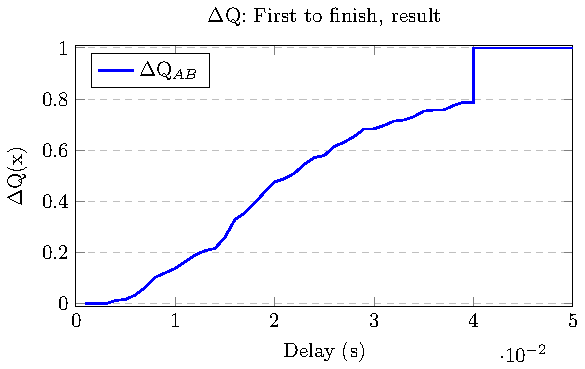
\includegraphics[scale = 0.7]{tikz/ftf_2.pdf}
                \label{fig:ftf2}
            \end{subfigure}
            \caption{Left: $\Delta$Q$_{(A, B)}$. Right: FTF$_{(A, B)}$ = $\Delta$Q$_{AB}$}%
            \label{fig:ftf}
            \end{figure}


    \subsubsection{All to finish (ATF)}
        If we assume two independent outcomes $O_A$, $O_B$ with the same start event, all-to-finish occurs when both end events occur, it can be calculated as:
        \begin{equation}
            \begin{split}
                \Delta Q_{ATF(A, B)} &= Pr[d_A \le t \wedge d_B \le t] \\
                & = Pr[d_A \le t] \cdot Pr[d_B \le t] = \Delta Q_A \cdot \Delta Q_B \\
                \Delta Q_{ATF(A, B)} &= \Delta Q_A \cdot \Delta Q_B 
            \end{split}
            \label{eq:atf}
        \end{equation}
        
        \begin{figure}[H]
            \centering
            \begin{subfigure}{.5\textwidth}
                \centering
                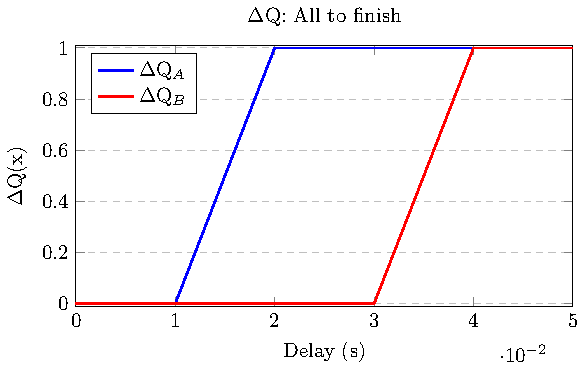
\includegraphics[scale = 0.7]{tikz/atf_1.pdf}
                \label{fig:atf_1}
            \end{subfigure}%
            \begin{subfigure}{.5\textwidth}
                \centering
                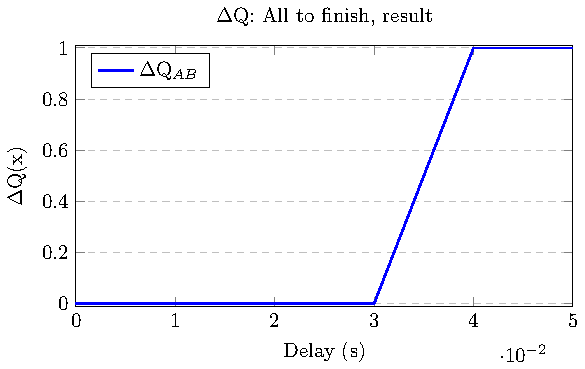
\includegraphics[scale = 0.7]{tikz/atf_2.pdf}
                \label{fig:atf2}
            \end{subfigure}
            \caption{Left: $\Delta$Q$_{(A, B)}$. Right: ATF$_{(A, B)}$ = $\Delta$Q$_{AB}$}%
            \label{fig:atf}
            \end{figure}

    \subsubsection{Probabilistic choice (PC)}
        If we assume two possible outcomes $O_A$ and $O_B$ and exactly one outcome is chosen during each occurence of a start event and:
        \begin{itemize}
            \item $O_A$ happens with probability $\dfrac{p}{p+q}$
            \item $O_B$ happens with probability $\dfrac{q}{p + q}$
        \end{itemize}
        \begin{equation}
           \Delta Q_{PC}(A, B) = \dfrac{p}{p + q}\Delta Q_A + \dfrac{q}{p + q}\Delta Q_B 
            \label{eq:pc}
        \end{equation} 

    \begin{figure}[H]
        \begin{center}
            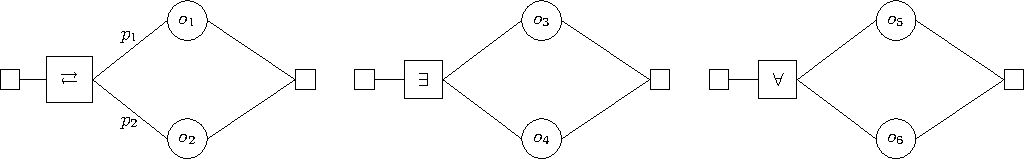
\includegraphics[width = \textwidth]{tikz/op.pdf}
        \end{center}
        \caption{The possible operators in an outcome diagram: Probabilistic choice, first-to-finish, all-to-finish}
        \label{fig:op}
    \end{figure}
    First-to-finish, All-to-finish and probabilistic-choice are calculated on the CDF of the $\Delta$Q of their components.
    
    These operators can be assembled together to create an outcome diagram, later on, we will see how one can go from the graphical representation to outcome diagrams which can be used in the $\Delta$Q oscilloscope.
    
    \subsection{Outcome diagrams refinement}
        An important feature of outcome diagrams is the ability to be able to design a system even with \textit{"black-boxes"}, before the complete details of it are known. \\
        An outcome diagram can be "unboxed" by refining the outcomes that compose it. We can adapt a situation described in Mind your Outcomes to understand how refinement can allow the user to have a very precise representation of a system. \cite{myo}
        
        We first start with a black-box, unnamed outcome with start event $A$ and end event $Z$, somewhere in the system. The first refinement step would be giving the outcome a name.

      \begin{figure}[H]
            \begin{center}
                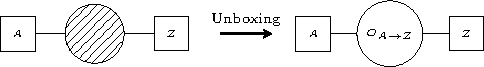
\includegraphics[scale = 1]{tikz/black_box.pdf}
            \end{center}
            \caption{Refinement from black box to named outcome.}
            \label{fig:bb}
        \end{figure}

    The system can be further refined by adding outcomes that represent tasks. For example, the engineer might believe that it will take two tasks to get from A to Z. We can then add another outcome, sequentially composed, to represent this situation.

       \begin{figure}[H]
            \begin{center}
                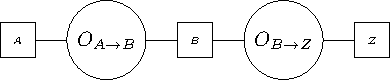
\includegraphics[scale = 1]{tikz/out_2.pdf}
            \end{center}
            \caption{Further refinement from one task to two tasks.}
            \label{fig:2_hops}
        \end{figure}

        We can also model the chance of executing two tasks as a probabilistic choice, where there is $p_2$ probability that the execution from A to Z will execute two tasks. The outcome diagram can be refined as a probabilistic choice.

   \begin{figure}[H]
            \begin{center}
                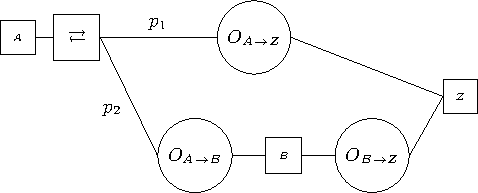
\includegraphics[scale = 1]{tikz/ref_op.pdf}
            \end{center}
            \caption{Refinement as probabilistic choice of executing either one or two tasks.}
            \label{fig:prob_ref}
        \end{figure}
    In essence, the refinement could model a very fine-grained representation of the system by further refining the system, to represent the possibility of executing $n$ tasks. This demonstrates the power of outcome diagrams to represent system diagrams with high precision. They can help explore design decisions thanks to outcomes and operators.

    \subsection{Independence hypothesis}  
        An important aspect of sequential composition is the assumption of outcomes having independent behaviour. Let us explain the following assumption clearly.

        Assume two sequentially composed outcomes $o_1$, $o_2$ running on the same processor. The overall delay of execution can be observed from the start event of $o_1$ ($u_1$) to the end event of $o_2$ ($r_1$). 
        \begin{figure}[H]
            \begin{center}
                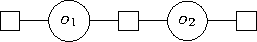
\includegraphics[scale=1]{tikz/indep.pdf}
            \end{center}
        \end{figure}
        
        At low load, the two components behavior will be independent, the system will behave \textbf{linearly}. According to the superposition principle, the overall delay will be the sum of the two delays, as will the overall processor utilisation. \cite{sup-p}
        
        When load increases, the two components will start to show dependent behaviour due to the processor utilisation increasing. The $\Delta$Q of the observed total delay will then deviate from the sum of the two delays ($o_1 \circledast o_2$). 
        
        \begin{figure}[H]
            \begin{center}
                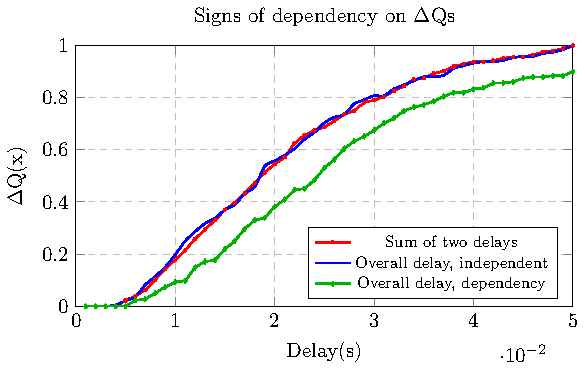
\includegraphics[scale=1]{tikz/cdf_indep.pdf}
            \end{center}
            \caption{When the components are independent, the sum of the two delays (blue) and the overall delay (red) can be superposed. \\
            When $o_1$ and $o_2$ show initial signs of dependency, the overall delay (green) can be seen deviating from the sum of the two delays.}
            \label{fig:cdf_indep}
        \end{figure}

        When the system is far from being overloaded, the effect is noticeable thanks to $\Delta$QSD. As the cliff edge of overload is approached, the nonlinearity will increase \cite{post}. These theoretical results can be observed in practice in the oscilloscope. We will explore such cases in the synthetic applications section.

    \section{Observability}
    OpenTelemetry refers to observability as \cite{otel-o}:
    \begin{quote}
 ``The ability to understand the internal state by examining its output. In the context of a distributed system, being able to understand the internal state of the system by examining its telemetry data.''
    \end{quote}
    In the case of the Erlang programming language, we describe respectively two different ways to observe a running Erlang system: erlang:trace and OpenTelemetry.
    
    \subsection{erlang:trace}
        The Erlang programming language gives the users different ways to observe the behaviour of a system, one of those is the interface \texttt{erlang:trace}. According to the documentation: ``The Erlang run-time system exposes several trace points that can be observed, observing the trace points allows users to be notified when they are triggered'' \cite{erl-t}. One can observe function calls, messages being sent and received, process being spawned, garbage collecting \dots. 
        \begin{figure}[!ht]
        \centering
        \begin{minted}{erlang}
            -spec trace(PidPortSpec, How, FlagList) -> integer()
               when
                   PidPortSpec ::
                       pid() |
                       port() |
                       all | processes | ports | existing | existing_processes | existing_ports | new |
                       new_processes | new_ports,
                   How :: boolean(),
                   FlagList :: [trace_flag()].
        \end{minted}
        \caption{erlang:trace/3 specification.}
\end{figure}

    Nevertheless, in Erlang trace there is no default way to follow a message and get its whole execution trace. This is a missing feature that is crucial for observing a program functioning and being able to connect an application to our oscilloscope.  This is where the OpenTelemetry framework comes in.

\subsection{OpenTelemetry}
    According to OpenTelemetry website \cite{otel-o}: OpenTelemetry is an open-source, vendor-agnostic observability framework and toolkit designed to generate, export and collect telemetry data, in particular traces, metrics and logs. OpenTelemetry provides a standard protocol, a single set of API and conventions and lets the user own the generated data, allowing to switch between observability backends freely.
   
   OpenTelemetry is available for a plethora of languages \cite{otel-l}, including Erlang, although, as of writing this, only traces are available in Erlang \cite{otel-in}.
     
    The Erlang Ecosystem Foundation has a working group focused on evolving the tools related to observability, including OpenTelemetry and the runtime observability monitoring tools \cite{obs-group}. 
    
    \subsubsection{Traces}
        Traces are why we are basing our program on top of OpenTelemetry, traces follow the whole path of a request in an application, and they are comprised of one or more spans. Traces can propagate to multiple services and record multiple paths in different microservices \cite{otel-dt}. 
        
        \paragraph{Span} A span is a unit of work or operation. Multiple spans can be assembled into a trace and can be causally linked (\cref{fig:monitor}). The spans can have a hierarchy, where \textit{root spans} represent a request from start to finish and a child span the requests that are completed inside the root span \cite{otel-dt}. We will see in later sections how this can relate to what the oscilloscope does.

    The notion of spans and traces allows us to follow the execution of a request and carry a context. Spans can be linked to mark causal relationships between multiple spans \cite{otel-t}. This relation can be represented in the oscilloscope via \textbf{probes}, we will present how spans relate to probes in following sections.
    \begin{figure}[H]
    \begin{minted}{json} 
{
  "name": "oscilloscope-span",
  "context": {
    "trace_id": "5b8aa5a2d2c872e8321cf37308d69df2",
    "span_id": "5fb397be34d26b51"
  },
  "parent_id": "051581bf3cb55c13",
  "start_time": "2022-04-29T18:52:58.114304Z",
  "end_time": "2022-04-29T22:52:58.114561Z",
  "attributes": {
    "http.route": "some_route"
  },
}
    \end{minted}
    \caption{Example of span from the OpenTelemetry website \cite{otel-t}. The span has a parent, indicating that child and parent spans are related and are both part of the same trace.}%
    \end{figure}

    \subsubsection{Monitoring OpenTelemetry spans}
        In OpenTelemetry, the user can export their traces export to backends and monitoring such as Jaeger (\cref{fig:monitor}), Zipkin, Datadog \cite{otel-exp}. There, a user can analyse the traces to troubleshoot their programs by observing the flow of the requests \cite{jg}. These monitoring tools give extensive details about a running system, but may fail to capture essential timeliness requirements and performances issues early enough.
        
        Our oscilloscope is a kind of monitoring tool, one that gives precise statistical insights about a running system. It is clear that the oscilloscope does not have the same capabilities as Datadog \cite{datadog} might have, where you can observe cloud instances, instances cost, dependency graphs \dots but the oscilloscope can nevertheless provide precise insights about dependency, overload thanks to the $\Delta$QSD paradigm. 

        This is also the reason why the adapter includes OpenTelemetry macros. The oscilloscope can be put next to a monitoring tool where one might export spans to, so that an engineer might consult the monitoring tool to get the global picture of a running app. The oscilloscope provides more precise insights to understand the system's behaviour. 
       \begin{figure}[H]
            \centering
            \begin{subfigure}{.5\textwidth}
                \centering
                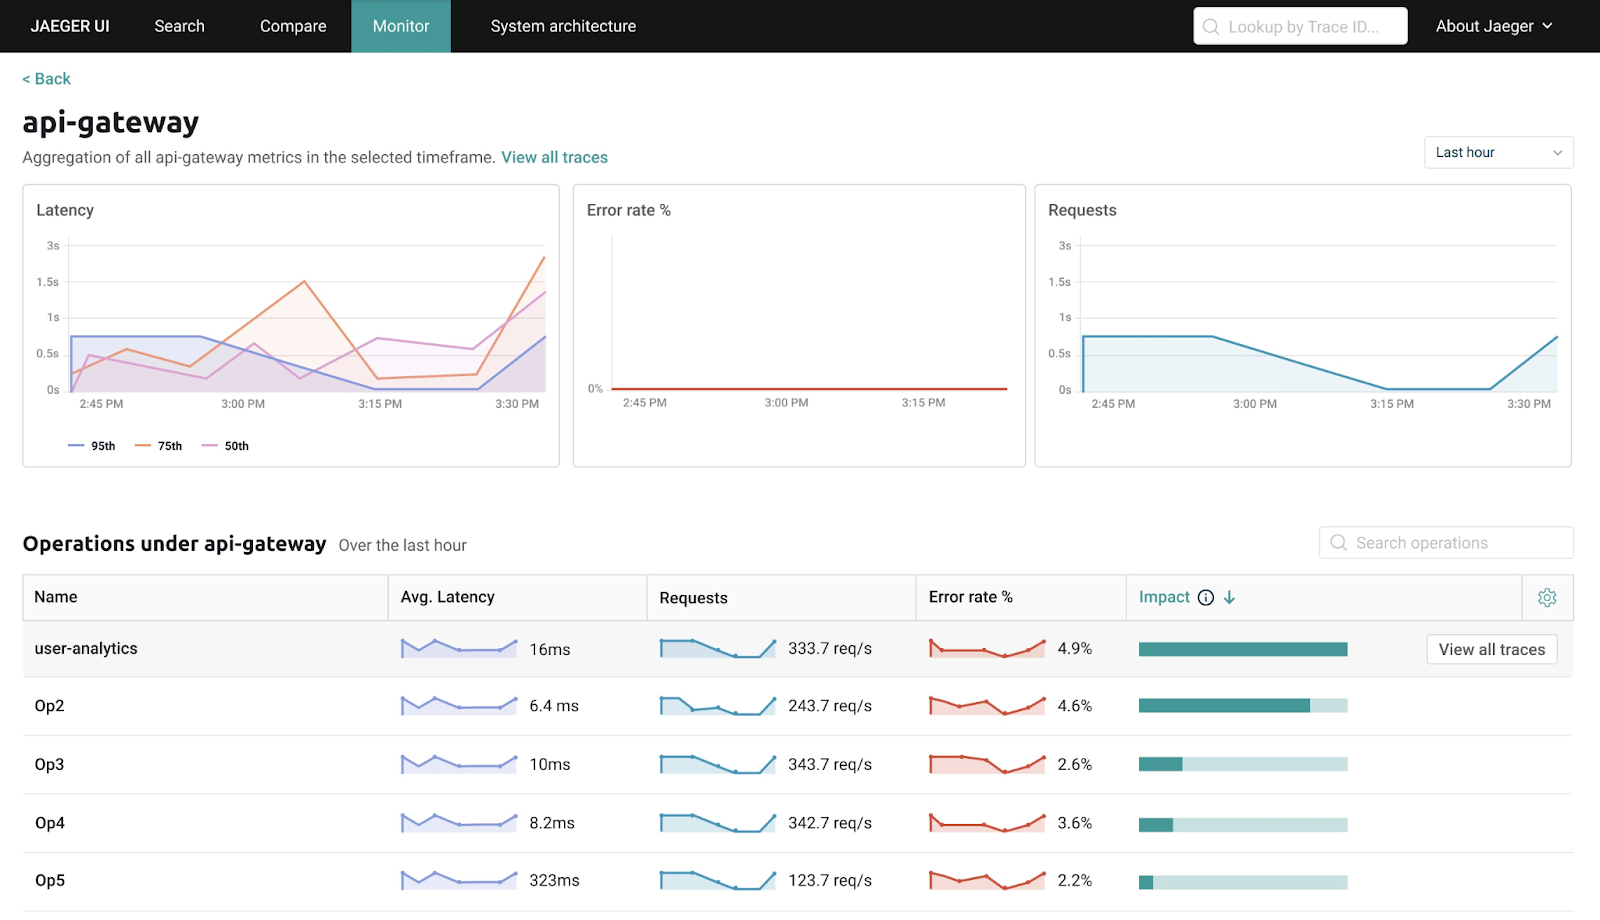
\includegraphics[width=0.98\textwidth]{img/jaeger.png}
                \label{fig:jag}
            \end{subfigure}%
            \begin{subfigure}{.5\textwidth}
                \centering
                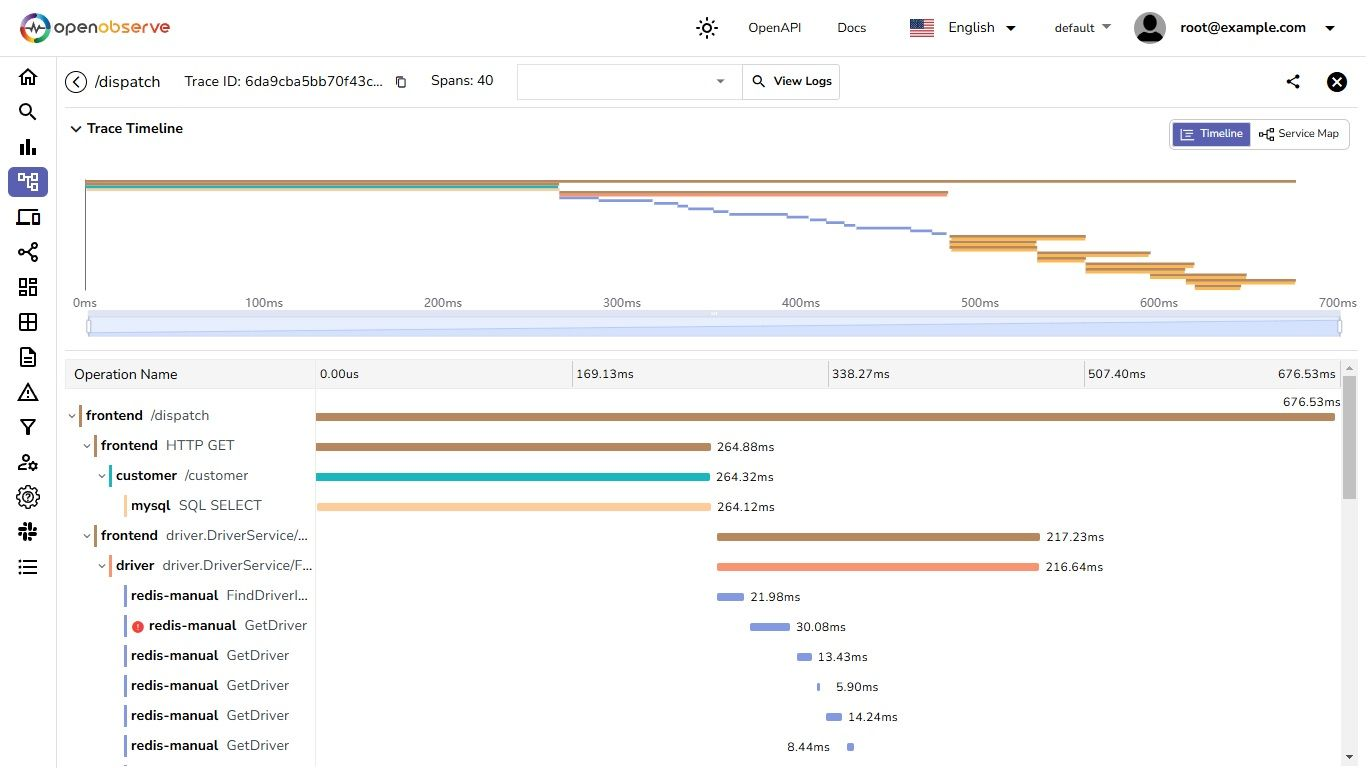
\includegraphics[width =0.98\textwidth]{img/jaeger2.jpg}
                \label{fig:openobs}
            \end{subfigure}
            \caption{Left: Jaeger interface. Right: Analysis of a span on OpenObserve.}
            \label{fig:monitor}
            \end{figure}

    \subsubsection{Span macros}
        OpenTelemetry provides macros to start, end and interact with spans in Erlang, the following code excerpts are taken from the OpenTelemetry instrumentation wiki. \cite{otel-in}
        \paragraph{?with\_span}
            \texttt{?with\_span} creates active spans. An active span is the span that is currently set in the execution context and is considered the ``current'' span for the ongoing operation or thread. \cite{active-s}
        \begin{minted}{erlang}
parent_function() ->
    ?with_span(parent, #{}, fun child_function/0).
child_function() ->
    %% this is the same process, so the span parent set as the active
    %% span in the with_span call above will be the active span in this function
    ?with_span(child, #{},
               fun() ->
                   %% do work here. when this function returns, child will complete.
               end).
        \end{minted}
        \paragraph{?start\_span}
            \texttt{?start\_span} creates a span which isn't connected to a particular process, it does not set the span as the current active span.
        \begin{minted}{erlang}
SpanCtx = ?start_span(child),
Ctx = otel_ctx:get_current(),
proc_lib:spawn_link(fun() ->
                        otel_ctx:attach(Ctx),
                        ?set_current_span(SpanCtx),
                        ?end_span(SpanCtx)
                    end),
        \end{minted}
        \paragraph{?end\_span}
            \texttt{?end\_span} ends a span started with \texttt{?start\_span}


    \section{Current observability problems}

    A legitimate question to pose would be why one would need an additional tool to observe their system, monitoring tools are already plenty and provide useful insights into an application's behaviour. While they may seem adequate to provide a global oversight of applications, they fail to diagnose real time problems like overload, dependent behaviour early enough and in a quick manner.

    The problem we are trying to tackle can be described by the following situation: 
    Imagine an Erlang application instrumented with OpenTelemetry, suddenly, the application starts slowing down, and the execution of a function takes 10 seconds instead of the usual 1 second. Between its start and its end, the user instrumenting the application sees nothing in their dashboard.
    
    This is a big problem! One would like to know right away if something is wrong with their application, better! Even before problems are apparent. This is where the $\Delta$QSD paradigm and the $\Delta$Q oscilloscope come in handy.
   
   By leveraging $\Delta$QSD notion of failure and QTAs, problems can be detected right away in the oscilloscope. 
    
    \begin{figure}[H]
        \begin{center}
            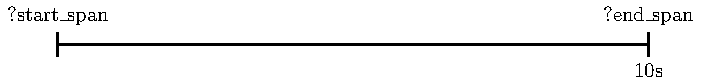
\includegraphics{tikz/start_end.pdf}
        \end{center}
        \caption{Execution of a long span in OpenTelemetry, the user will only be notified after 10 seconds that the function has ended (and taken too long).}
    \end{figure}

    \begin{figure}[H]
        \begin{center}
            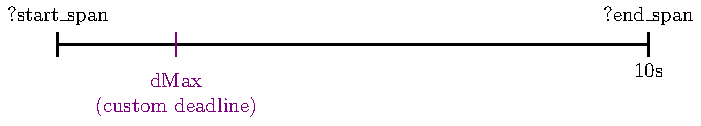
\includegraphics{tikz/start_end_dmax.pdf}
        \end{center}
        \caption{Execution of a long span in OpenTelemetry, the $dMax$ deadline allows knowing that the span has taken too long.}
        \label{fig:otel_dmax}
    \end{figure} 


    \subsection{Handling of long spans}
        OpenTelemetry presents a bigger problem, what happens when there are long-running spans? Worse, what happens when spans are not actually terminated?
        
        OpenTelemetry limits the length of its spans, moreover, those who are not terminated are lost and not exported. Why? Failed executions are those that tell more about a program's execution!

        If the span is the parent/root span, its effect could trickle down to child spans. We can quickly see how this becomes problematic, all the information about an execution of your program \dots lost. Moreover, a span could not be terminated for trivial reasons: refreshing a tab, network failures, crashes \dots \cite{otel-l}. There are a few hacks that can be implemented, having shorter spans, carrying data in child spans, saving spans in a log to track spans which were not ended to manually set an end time; why the need to circumvent limitations when observing a system?

     We believe that the adapter we provide can be a great start to improve observability requirements surrounding OpenTelemetry. We will show in the evaluation on synthetic applications how $\Delta$QSD's notion of failure can help to detect overload problems in running systems right away.

